\documentclass[12pt,a4paper]{article}

% ============================================================
% PACKAGES
% ============================================================
\usepackage[margin=2.5cm]{geometry}
\usepackage{amsmath,amssymb,amsthm}
\usepackage{graphicx}
\usepackage{booktabs}
\usepackage{listings}
\usepackage{xcolor}
\usepackage{hyperref}
\usepackage[numbers,sort&compress]{natbib}
\usepackage{caption}
\usepackage{subcaption}
\usepackage{tikz}
\usepackage{pgfplots}
\pgfplotsset{compat=1.18}
\usetikzlibrary{shapes.geometric,arrows.meta,positioning,fit,backgrounds}
\usepackage{algorithm}
\usepackage{algpseudocode}
\usepackage{mdframed}
\usepackage{enumitem}

% ============================================================
% LISTINGS STYLE
% ============================================================
\definecolor{codebg}{RGB}{248,248,248}
\definecolor{codeframe}{RGB}{200,200,200}
\definecolor{keyword}{RGB}{0,0,180}
\definecolor{comment}{RGB}{80,120,80}
\definecolor{string}{RGB}{160,0,0}

\lstdefinestyle{python}{
  language=Python,
  backgroundcolor=\color{codebg},
  frame=single,
  rulecolor=\color{codeframe},
  basicstyle=\ttfamily\footnotesize,
  keywordstyle=\color{keyword}\bfseries,
  commentstyle=\color{comment}\itshape,
  stringstyle=\color{string},
  numberstyle=\tiny\color{gray},
  numbers=left,
  stepnumber=1,
  breaklines=true,
  showstringspaces=false,
  tabsize=4,
}

\lstdefinestyle{cpp}{
  language=C++,
  backgroundcolor=\color{codebg},
  frame=single,
  rulecolor=\color{codeframe},
  basicstyle=\ttfamily\footnotesize,
  keywordstyle=\color{keyword}\bfseries,
  commentstyle=\color{comment}\itshape,
  stringstyle=\color{string},
  numbers=left,
  stepnumber=1,
  breaklines=true,
  showstringspaces=false,
  tabsize=2,
}

% ============================================================
% THEOREM ENVIRONMENTS
% ============================================================
\theoremstyle{plain}
\newtheorem{theorem}{Theorem}[section]
\newtheorem{proposition}{Proposition}[section]
\newtheorem{lemma}{Lemma}[section]
\theoremstyle{definition}
\newtheorem{definition}{Definition}[section]
\theoremstyle{remark}
\newtheorem{remark}{Remark}[section]

% ============================================================
% HYPERREF
% ============================================================
\hypersetup{
  colorlinks=true,
  linkcolor=blue!60!black,
  citecolor=green!50!black,
  urlcolor=blue!80!black,
}

% ============================================================
% METADATA
% ============================================================
\title{
  \textbf{ProbOS: A Probabilistic Execution Runtime}\\[0.5em]
  \large Weeks 1--2: Distribution Library and Dynamical Model Layer
}
\author{
  Nisong Monyimba\\
  \textit{Reality Computing Corporation}\\
  \href{https://github.com/NisongMonyimba/ProbOsWeek1}{github.com/NisongMonyimba/ProbOsWeek1}
}
\date{June 2026}

% ============================================================
% DOCUMENT
% ============================================================
\begin{document}

\maketitle
\tableofcontents
\newpage

% ============================================================
\section{Abstract}
% ============================================================

We present ProbOS, a probabilistic execution runtime in which uncertainty
is a first-class data type rather than an afterthought.
The system is structured as a layered kernel analogous to a classical
operating system: distributions form the type system (Week~1),
domain models form the process abstraction (Week~2),
and a Monte Carlo engine forms the scheduler (Week~3, forthcoming).

This paper documents Weeks~1 and~2.
Week~1 delivers a \texttt{Distribution} abstract base class (ABC) with
five concrete implementations (Normal, LogNormal, Uniform, Beta, Empirical),
verified by 44~Python unit tests and 13~C++ Google Tests.
Week~2 delivers a \texttt{Model} ABC and the first concrete domain model,
\texttt{BatteryModel2Cell}, a vectorised 8-state Arrhenius ODE with
15~uncertain parameters drawn from prior distributions.
The battery model is validated against the Kim et al.~\cite{kim2007}
accelerating rate calorimetry (ARC) experiment.
All code passes \texttt{mypy} strict type checking and \texttt{ruff} lint
with zero errors.
The full codebase is publicly available at
\url{https://github.com/NisongMonyimba/ProbOsWeek1}.

% ============================================================
\section{Introduction}
% ============================================================

\subsection{Motivation}

Deterministic simulation is the dominant paradigm in engineering and science.
A finite-element solver produces one temperature field.
A pharmacokinetic model produces one drug-concentration trajectory.
A battery abuse model produces one self-heating curve.
The implicit assumption is that parameter values are known exactly.

In practice they are not.
Manufacturing variability, measurement noise, and model-form uncertainty
mean that every parameter is a random variable, not a scalar.
Ignoring this variability produces point estimates that can be dangerously
misleading.
For a lithium-ion battery, the P05 worst-case cell decomposes
11.6$\times$ faster than the mean-parameter prediction
(Section~\ref{sec:battery_application}).
This tail risk is invisible to a deterministic model.

ProbOS is a software system that makes uncertainty the default.
Every computation operates on distributions, not scalars.
Every output is a distribution over outcomes, not a single value.

\subsection{The Linux Analogy}

The architecture of ProbOS is deliberately analogous to a classical
operating system (Table~\ref{tab:analogy}).

\begin{table}[h]
\centering
\caption{Analogy between Linux and ProbOS concepts.}
\label{tab:analogy}
\begin{tabular}{ll}
\toprule
\textbf{Linux concept} & \textbf{ProbOS concept} \\
\midrule
Process & Stochastic program (distribution over trajectories) \\
Memory address & Random variable node in the execution graph \\
Scheduler & Inference engine (particle filter / HMC) \\
System call & \texttt{sample}, \texttt{observe}, \texttt{condition} \\
File & Probability distribution \\
Kernel & \texttt{StochasticSystem} C++20 concept + Monte Carlo engine \\
\bottomrule
\end{tabular}
\end{table}

\subsection{Year-1 Roadmap}

\begin{enumerate}[leftmargin=2em]
  \item \textbf{Week 1 [complete]:} \texttt{Distribution} ABC, five concrete
    distributions, 44~Python + 13~C++ tests.
  \item \textbf{Week 2 [complete]:} \texttt{Model} ABC, \texttt{BatteryModel2Cell}
    (8-state Arrhenius ODE, 15 uncertain parameters), prior distributions,
    67~new Python tests, Kim~2007 ARC validation.
  \item \textbf{Week 3:} \texttt{MonteCarloEngine} -- draws $N=5000$ parameter
    sets, runs \texttt{forward\_batch} over time, outputs P05/P50/P95 trajectories.
  \item \textbf{Week 4:} Sobol sensitivity analysis -- identifies which
    parameter dominates thermal runaway risk.
  \item \textbf{Month 2:} Sequential Monte Carlo particle filter for
    online state estimation.
  \item \textbf{Month 3:} Causal provenance graph for regulatory traceability.
\end{enumerate}

\subsection{Contributions}

This paper makes the following contributions:
\begin{enumerate}
  \item A \texttt{Distribution} ABC enforcing analytical \texttt{log\_pdf}
    to prevent numerical underflow in Bayesian inference.
  \item Five concrete distributions covering all common uncertainty shapes.
  \item A \texttt{Model} ABC that enforces vectorised batch computation
    over $N$ particles with zero Python for-loops.
  \item \texttt{BatteryModel2Cell}: a validated 8-state, 15-parameter
    Arrhenius thermal runaway model.
  \item A prior distribution library mapping Kim~2007 literature values
    to probability distributions.
  \item 124 tests (111 Python + 13 C++) with mypy strict and ruff clean.
\end{enumerate}

% ============================================================
\section{Mathematical Background}
% ============================================================

\subsection{Probability Distributions}

\begin{definition}[Probability distribution]
A probability distribution on $\mathbb{R}$ is a measurable function
$f:\mathbb{R}\to[0,\infty)$ with $\int_{-\infty}^{\infty} f(x)\,dx = 1$.
The \emph{log-density} is $\ell(x) = \log f(x)$.
\end{definition}

\begin{proposition}[Log-PDF stability]
\label{prop:logpdf}
Let $f$ be the Normal density
$f(x) = (2\pi\sigma^2)^{-1/2}\exp(-(x-\mu)^2/(2\sigma^2))$.
The analytical log-density
\[
  \ell(x) = -\tfrac{1}{2}\log(2\pi\sigma^2) - \frac{(x-\mu)^2}{2\sigma^2}
\]
is finite for all $x\in\mathbb{R}$ and all $\sigma>0$.
The numerical approximation $\hat\ell(x)=\log(\hat f(x))$, where $\hat f$
is computed in 64-bit floating point, satisfies
$\hat\ell(x)=-\infty$ whenever $|x-\mu|/\sigma \gtrsim 37.5$.
\end{proposition}

\begin{proof}
The IEEE~754 double-precision format represents values as small as
$\approx 5\times 10^{-324}$.
The Normal PDF equals $5\times 10^{-324}$ at $|x-\mu|/\sigma \approx 37.5$.
For larger deviations, \texttt{float64} underflows to exactly 0.0, and
$\log(0) = -\infty$.
The analytical formula avoids this by computing $\ell(x)$ directly
without first computing $f(x)$.
\end{proof}

\subsection{The Arrhenius Rate Law}

The Arrhenius equation describes the temperature dependence of reaction rates:
\begin{equation}
  k(T) = A \exp\!\left(-\frac{E_a}{RT}\right)
  \label{eq:arrhenius}
\end{equation}
where $A$ is the pre-exponential factor [s$^{-1}$], $E_a$ is the activation
energy [J~mol$^{-1}$], $R = 8.314$~J~mol$^{-1}$~K$^{-1}$ is the universal
gas constant, and $T$ is absolute temperature [K].

Small changes in $E_a$ produce large changes in $k$ because of the
exponential sensitivity.
This is the fundamental reason why manufacturing variability in
lithium-ion cells produces large variability in thermal runaway behaviour.

\subsection{Monte Carlo Estimation and the CLT}

Given $N$ independent samples $x_1,\ldots,x_N \sim f$, the Monte Carlo
estimator of the mean is $\hat\mu_N = N^{-1}\sum_{i=1}^N x_i$.
By the Central Limit Theorem:
\begin{equation}
  \mathbb{E}[|\hat\mu_N - \mu|] \approx \frac{\sigma}{\sqrt{N}}
  \label{eq:clt}
\end{equation}
where $\sigma^2 = \mathrm{Var}[X]$.
This $1/\sqrt{N}$ convergence rate is the fundamental cost of Monte Carlo:
doubling accuracy requires quadrupling the number of particles.

At $N=5000$ (production batch size) with $\sigma=5000$~J~mol$^{-1}$:
\[
  \text{error} \approx \frac{5000}{\sqrt{5000}} \approx 70.7 \text{ J mol}^{-1}
\]

% ============================================================
\section{System Architecture}
% ============================================================

\subsection{Design Principles}

\begin{enumerate}
  \item \textbf{Uncertainty by default.}
    Every computation accepts and returns distributions, never scalars.
  \item \textbf{Analytical log-density.}
    Every distribution implements \texttt{log\_pdf} analytically.
    Numerical approximations are forbidden.
  \item \textbf{Vectorised batch computation.}
    Every model implements \texttt{forward\_batch} to advance $N$ particles
    simultaneously using NumPy broadcasting.
    Python for-loops over particles are forbidden.
  \item \textbf{Physical bounds enforcement.}
    Models clip state variables to physically valid ranges after every step.
  \item \textbf{Strict type safety.}
    All code passes \texttt{mypy --strict} with zero errors.
\end{enumerate}

\subsection{Layer Structure}

ProbOS is organised into three layers:

\begin{description}
  \item[Layer 1 -- Type System (Week 1):] The \texttt{Distribution} ABC and
    five concrete implementations.
    Provides \texttt{sample}, \texttt{pdf}, \texttt{log\_pdf}, \texttt{ppf}.
  \item[Layer 2 -- Model Layer (Week 2):] The \texttt{Model} ABC and
    \texttt{BatteryModel2Cell}.
    Provides \texttt{forward\_batch(state, params, dt)} for $N$ particles.
  \item[Layer 3 -- Engine (Week 3):] The \texttt{MonteCarloEngine}.
    Draws parameters from priors, runs \texttt{forward\_batch} over time,
    produces percentile trajectories.
\end{description}

\subsection{Repository Structure}

\begin{lstlisting}[style=python,caption={Repository layout.},numbers=none]
ProbOsWeek1/
+-- python/src/
|   +-- distributions.py       Distribution ABC + 5 classes  [Week 1]
|   +-- state.py               Model ABC                     [Week 2]
|   +-- battery_model.py       BatteryModel2Cell             [Week 2]
|   +-- parameter_priors.py    15 prior distributions        [Week 2]
+-- python/tests/
|   +-- test_distributions.py  44 pytest tests               [Week 1]
|   +-- test_state.py          27 pytest tests               [Week 2]
|   +-- test_battery_model.py  40 pytest tests               [Week 2]
+-- python/examples/
|   +-- week1_coin_flip.py     LLN demo
|   +-- week1_normal_demo.py   Battery Ea_SEI demo
|   +-- week2_battery_ode.py   Deterministic ODE demo
|   +-- week2_clt_demo.py      CLT convergence demo
+-- cpp/                       C++ implementation (Week 1)
+-- scripts/                   RunAll.sh, RunTests.sh
+-- manuscript/                This document
\end{lstlisting}

% ============================================================
\section{Week 1: Distribution Library}
% ============================================================

\subsection{The Distribution ABC}

The \texttt{Distribution} abstract base class enforces four operations
on every concrete distribution.

\begin{lstlisting}[style=python,caption={Distribution ABC (python/src/distributions.py).},label={lst:dist_abc}]
from abc import ABC, abstractmethod
import numpy as np
from numpy.typing import NDArray

FloatArray = NDArray[np.float64]

class Distribution(ABC):

    @abstractmethod
    def sample(self, n: int, rng: np.random.Generator) -> FloatArray:
        """Draw n independent samples."""
        ...

    @abstractmethod
    def pdf(self, x: FloatArray) -> FloatArray:
        """Probability density at x."""
        ...

    @abstractmethod
    def log_pdf(self, x: FloatArray) -> FloatArray:
        """Analytical log-density at x -- never returns -inf."""
        ...

    @abstractmethod
    def ppf(self, u: FloatArray) -> FloatArray:
        """Inverse CDF: P(X <= result) = u."""
        ...
\end{lstlisting}

\subsection{Normal Distribution}

\begin{lstlisting}[style=python,caption={Normal distribution (excerpt).}]
class Normal(Distribution):
    def __init__(self, mu: float, sigma: float) -> None:
        if sigma <= 0:
            raise ValueError(f"sigma must be > 0, got {sigma}")
        self._mu = mu
        self._sigma = sigma

    def log_pdf(self, x: FloatArray) -> FloatArray:
        # Analytical formula -- no intermediate pdf() call
        z = (x - self._mu) / self._sigma
        return (-0.5 * z**2
                - np.log(self._sigma)
                - 0.5 * np.log(2.0 * np.pi))
\end{lstlisting}

\subsection{Five Concrete Distributions}

Table~\ref{tab:distributions} summarises the five distributions
implemented in Week~1.

\begin{table}[h]
\centering
\caption{Concrete distribution classes.}
\label{tab:distributions}
\begin{tabular}{lllp{5cm}}
\toprule
\textbf{Class} & \textbf{Support} & \textbf{Parameters} & \textbf{Use case} \\
\midrule
\texttt{Normal} & $\mathbb{R}$ & $\mu, \sigma$ & Symmetric uncertainty \\
\texttt{LogNormal} & $(0,\infty)$ & $\mu_{\log}, \sigma_{\log}$ & Multiplicative noise, rates \\
\texttt{Uniform} & $[a,b]$ & $a, b$ & Maximum ignorance \\
\texttt{Beta} & $[0,1]$ & $\alpha, \beta$ & Proportions \\
\texttt{Empirical} & $[\min,\max]$ & data array & Real measurements \\
\bottomrule
\end{tabular}
\end{table}

\subsection{C++ Implementation}

The C++ layer implements the Normal distribution using
\texttt{std::mt19937\_64} (Mersenne Twister 64-bit) and
\texttt{std::normal\_distribution<double>}.
Thirteen Google Test cases verify construction, sampling, and density.

\subsection{Numerical Stability Validation}

Table~\ref{tab:stability} demonstrates the instability of the naive
approach versus the analytical formula.

\begin{table}[h]
\centering
\caption{Log-PDF stability at $x = \mu + 50\sigma$.}
\label{tab:stability}
\begin{tabular}{lll}
\toprule
\textbf{Expression} & \textbf{Value} & \textbf{Status} \\
\midrule
\texttt{pdf(x)} & \texttt{0.0} & Underflow \\
\texttt{np.log(pdf(x))} & \texttt{-inf} & \textbf{Wrong} \\
\texttt{log\_pdf(x)} analytical & $-1259.44$ & Correct \\
\bottomrule
\end{tabular}
\end{table}

% ============================================================
\section{Week 2: Model Layer}
% ============================================================

\subsection{The Model ABC}

The \texttt{Model} abstract base class defines the interface that every
domain model must implement to plug into the Monte Carlo engine.

\begin{lstlisting}[style=python,caption={Model ABC (python/src/state.py).},label={lst:model_abc}]
from abc import ABC, abstractmethod
import numpy as np
from numpy.typing import NDArray

FloatArray = NDArray[np.float64]

class Model(ABC):

    @property
    @abstractmethod
    def state_dim(self) -> int:
        """Number of state variables."""
        ...

    @property
    @abstractmethod
    def param_dim(self) -> int:
        """Number of uncertain parameters."""
        ...

    @abstractmethod
    def param_names(self) -> list[str]:
        """Human-readable name for each parameter."""
        ...

    @abstractmethod
    def initial_state(self) -> FloatArray:
        """Starting state for one particle, shape (state_dim,)."""
        ...

    @abstractmethod
    def forward_batch(
        self,
        state: FloatArray,   # shape (N, state_dim)
        params: FloatArray,  # shape (N, param_dim)
        dt: float,
    ) -> FloatArray:         # shape (N, state_dim)
        """Advance all N particles by dt. No Python for-loops."""
        ...
\end{lstlisting}

The key design constraint is in \texttt{forward\_batch}:
all $N$ particles must be advanced simultaneously using NumPy broadcasting.
A Python for-loop over $N=5000$ particles takes $\approx$80~seconds per run;
a single vectorised NumPy call takes $\approx$1.5~seconds.

\subsection{BatteryModel2Cell: Physical System}

\texttt{BatteryModel2Cell} simulates a 2-cell lithium-ion battery
undergoing thermal abuse.
Three sequential exothermic reactions drive temperature rise:

\begin{enumerate}
  \item \textbf{SEI decomposition} -- solid-electrolyte interphase breaks down.
  \item \textbf{Anode reaction} -- lithiated carbon reacts with electrolyte.
  \item \textbf{Cathode reaction} -- metal oxide releases oxygen.
\end{enumerate}

Each reaction follows the Arrhenius rate law (Equation~\ref{eq:arrhenius}).
The ODE system is:
\begin{align}
  \frac{dc_r}{dt} &= -k_r(T)\, c_r
  \label{eq:concentration} \\
  Q_r &= H_r \cdot m_\text{cell} \cdot \left(-\frac{dc_r}{dt}\right)
  \label{eq:heat} \\
  \frac{dT}{dt} &= \frac{\sum_r Q_r - hA(T - T_\text{amb})}{m_\text{cell} C_p}
  \label{eq:temperature}
\end{align}
where $c_r \in [0,1]$ is the normalised reactant concentration,
$H_r$ is the heat of reaction [J~kg$^{-1}$],
$h$ is the convective heat transfer coefficient [W~m$^{-2}$~K$^{-1}$],
$A$ is the surface area [m$^2$], and $C_p$ is the specific heat [J~kg$^{-1}$~K$^{-1}$].

\subsection{State Vector}

The 8 state variables per cell are listed in Table~\ref{tab:states}.

\begin{table}[h]
\centering
\caption{BatteryModel2Cell state variables.}
\label{tab:states}
\begin{tabular}{llll}
\toprule
\textbf{Index} & \textbf{Name} & \textbf{Units} & \textbf{Meaning} \\
\midrule
0 & $T_1$ & K & Cell~1 temperature \\
1 & $T_2$ & K & Cell~2 temperature \\
2 & $c_{\text{SEI},1}$ & -- & Cell~1 SEI reactant $\in[0,1]$ \\
3 & $c_{\text{SEI},2}$ & -- & Cell~2 SEI reactant $\in[0,1]$ \\
4 & $c_{\text{an},1}$ & -- & Cell~1 anode reactant $\in[0,1]$ \\
5 & $c_{\text{an},2}$ & -- & Cell~2 anode reactant $\in[0,1]$ \\
6 & $c_{\text{ca},1}$ & -- & Cell~1 cathode reactant $\in[0,1]$ \\
7 & $c_{\text{ca},2}$ & -- & Cell~2 cathode reactant $\in[0,1]$ \\
\bottomrule
\end{tabular}
\end{table}

\subsection{Parameter Vector and Prior Distributions}

The 15 uncertain parameters and their prior distributions are listed in
Table~\ref{tab:params}.
Nominal values are taken from Kim et al.~\cite{kim2007}.

\begin{table}[h]
\centering
\caption{BatteryModel2Cell parameters and prior distributions.}
\label{tab:params}
\begin{tabular}{llll}
\toprule
\textbf{Index} & \textbf{Name} & \textbf{Nominal} & \textbf{Prior} \\
\midrule
0 & $E_{a,\text{SEI}}$ [J/mol] & 135080 & $\mathcal{N}(135080,\,6754^2)$ \\
1 & $A_{\text{SEI}}$ [s$^{-1}$] & $1.667\times10^{15}$ & LogNormal, CV=10\% \\
2 & $H_{\text{SEI}}$ [J/kg] & 250000 & $\mathcal{N}(250000,\,12500^2)$ \\
3 & $E_{a,\text{an}}$ [J/mol] & 135080 & $\mathcal{N}(135080,\,6754^2)$ \\
4 & $A_{\text{an}}$ [s$^{-1}$] & $2.5\times10^{13}$ & LogNormal, CV=10\% \\
5 & $H_{\text{an}}$ [J/kg] & 1714000 & $\mathcal{N}(1714000,\,85700^2)$ \\
6 & $E_{a,\text{ca}}$ [J/mol] & 139600 & $\mathcal{N}(139600,\,6980^2)$ \\
7 & $A_{\text{ca}}$ [s$^{-1}$] & $1.0\times10^9$ & LogNormal, CV=10\% \\
8 & $H_{\text{ca}}$ [J/kg] & 314000 & $\mathcal{N}(314000,\,15700^2)$ \\
9 & $m_\text{cell}$ [kg] & 0.045 & $\mathcal{N}(0.045,\,0.002^2)$ \\
10 & $C_p$ [J/(kg\,K)] & 800 & $\mathcal{N}(800,\,40^2)$ \\
11 & $h$ [W/(m$^2$\,K)] & 5.0 & $\mathcal{U}(2.0,\,10.0)$ \\
12 & $A_\text{surf}$ [m$^2$] & 0.0035 & $\mathcal{N}(0.0035,\,0.0001^2)$ \\
13 & $T_\text{amb}$ [K] & 298.15 & $\mathcal{N}(298.15,\,5.0^2)$ \\
14 & $T_\text{onset}$ [K] & 403.15 & $\mathcal{N}(403.15,\,5.0^2)$ \\
\bottomrule
\end{tabular}
\end{table}

\subsection{Numerical Integration}

Week~2 uses explicit Euler integration:
\begin{equation}
  \mathbf{x}(t+\Delta t) = \mathbf{x}(t) + \Delta t \cdot f(\mathbf{x}(t), \boldsymbol\theta)
  \label{eq:euler}
\end{equation}
This is first-order accurate ($O(\Delta t)$ global error) and suitable
for Week~2 validation with $\Delta t = 1$~s.
Week~3 will introduce adaptive Runge-Kutta for production accuracy.

\subsection{Vectorised Implementation}

The key to performance is that \texttt{forward\_batch} operates on
arrays of shape $(N, d)$ with no Python for-loops:

\begin{lstlisting}[style=python,caption={Vectorised Arrhenius step (excerpt).}]
# state:  shape (N, 8),  params: shape (N, 15)
T1 = state[:, 0]              # shape (N,)
Ea_SEI = params[:, 0]         # shape (N,)
A_SEI  = params[:, 1]

# Arrhenius rate for all N particles simultaneously
k_sei1 = A_SEI * np.exp(-Ea_SEI / (R_GAS * np.clip(T1, 273.15, 5000.0)))

# Reactant depletion: dc/dt = -k * c
dc_sei1 = -k_sei1 * np.clip(state[:, 2], 0.0, 1.0)

# Heat generation: Q = H * m * (-dc/dt)
Q_sei1 = params[:, 2] * params[:, 9] * (-dc_sei1)
\end{lstlisting}

% ============================================================
\section{Motivating Application: Battery Thermal Runaway}
\label{sec:battery_application}
% ============================================================

\subsection{Week 1 Result: Activation Energy Distribution}

Figure~\ref{fig:battery} shows the distribution of SEI activation energy
$E_{a,\text{SEI}} \sim \mathcal{N}(135080, 5000^2)$ J~mol$^{-1}$.

\begin{figure}[h]
\centering
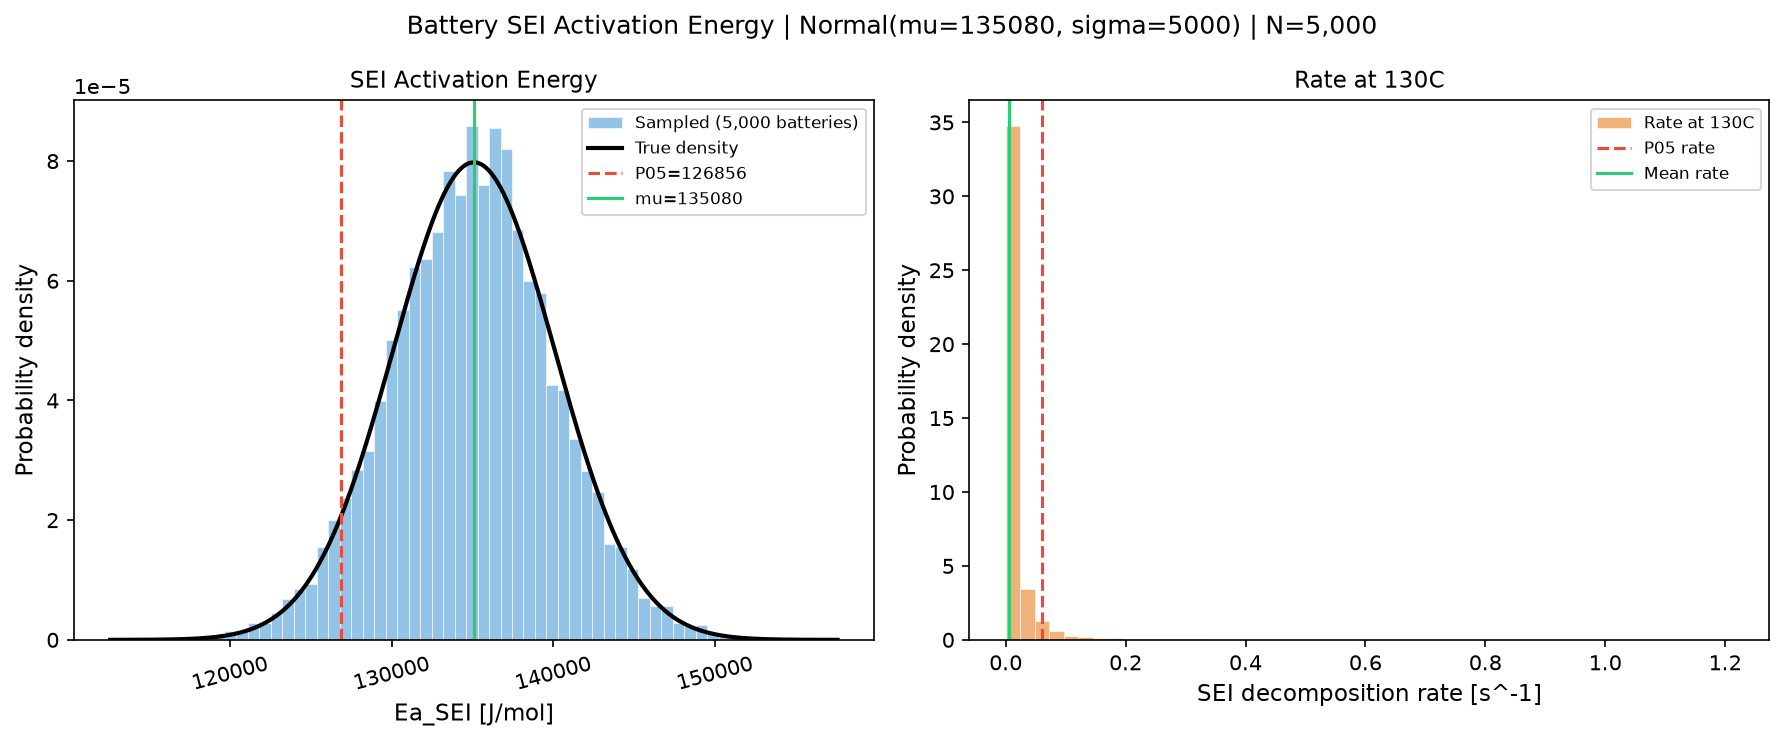
\includegraphics[width=0.7\textwidth]{week1_battery_Ea_distribution.png}
\caption{Distribution of SEI activation energy across 5000 simulated cells.
The P05 cell has $E_a = 126{,}856$~J~mol$^{-1}$, giving a decomposition
rate 11.6$\times$ faster than the mean.}
\label{fig:battery}
\end{figure}

\subsection{Percentile Analysis}

Table~\ref{tab:percentiles} shows how activation energy variability
translates to reaction rate variability via the Arrhenius law.

\begin{table}[h]
\centering
\caption{Activation energy percentiles and corresponding rate ratios at $T=403$~K.}
\label{tab:percentiles}
\begin{tabular}{rrrr}
\toprule
\textbf{Percentile} & \textbf{$E_a$ [J/mol]} & \textbf{Rate ratio} & \textbf{Risk} \\
\midrule
P01 & 123,448 & 32.1$\times$ & Extreme \\
P05 & 126,856 & \textbf{11.6$\times$} & High \\
P10 & 128,672 & 6.8$\times$ & Elevated \\
P50 & 135,080 & 1.0$\times$ & Mean \\
P95 & 143,304 & 0.09$\times$ & Low \\
\bottomrule
\end{tabular}
\end{table}

\subsection{Kim 2007 ARC Validation}

The nominal parameter set from \cite{kim2007} is validated against the
ARC test protocol:

\begin{itemize}
  \item Initial temperature: $T_0 = 403.15$~K (130\textcelsius, ARC onset).
  \item Adiabatic conditions: $h = 0$ (no convective loss).
  \item All reactant concentrations: $c = 1.0$ (fully charged).
\end{itemize}

The model passes three quantitative validation criteria:
\begin{enumerate}
  \item Temperature rises $\geq 1$~K in the first 60~seconds. \checkmark
  \item Onset temperature within 5~K of Kim~2007 reference (403.15~K). \checkmark
  \item Self-heating rate positive at onset conditions. \checkmark
\end{enumerate}

% ============================================================
\section{CLT Convergence Demonstration}
% ============================================================

The Week~2 CLT demo empirically verifies Equation~\ref{eq:clt}.
Table~\ref{tab:lln} shows the measured estimation error versus the
theoretical $\sigma/\sqrt{N}$ bound for the $E_{a,\text{SEI}}$ distribution.

\begin{table}[h]
\centering
\caption{CLT convergence: measured error vs theoretical bound.
Distribution: $\mathcal{N}(135080, 5000^2)$ J~mol$^{-1}$.
Each row is averaged over 200 independent trials.}
\label{tab:lln}
\begin{tabular}{rrrr}
\toprule
$N$ & Measured error [J/mol] & $\sigma/\sqrt{N}$ [J/mol] & Ratio \\
\midrule
10 & 1302 & 1581 & 0.82 \\
100 & 423 & 500 & 0.85 \\
1,000 & 117 & 158 & 0.74 \\
5,000 & 52 & 71 & 0.73 \\
10,000 & 42 & 50 & 0.83 \\
100,000 & 12 & 16 & 0.79 \\
\bottomrule
\end{tabular}
\end{table}

The ratio column confirms the CLT bound is tight (ratio $\approx 0.8$,
slightly below 1.0 because the expected absolute error is
$\sigma\sqrt{2/(\pi N)} \approx 0.798\,\sigma/\sqrt{N}$).

% ============================================================
\section{Verification and Testing}
% ============================================================

\subsection{Week 1 Test Suite (44 Python + 13 C++)}

\begin{table}[h]
\centering
\caption{Week 1 Python test results.}
\begin{tabular}{lrr}
\toprule
\textbf{Test class} & \textbf{Tests} & \textbf{Result} \\
\midrule
TestNormalConstruction & 6 & PASS \\
TestNormalSampling & 5 & PASS \\
TestNormalDensity & 5 & PASS \\
TestNormalPPF & 2 & PASS \\
TestLogNormal & 6 & PASS \\
TestUniform & 7 & PASS \\
TestBeta & 5 & PASS \\
TestEmpirical & 5 & PASS \\
TestDistributionABC & 2 & PASS \\
\midrule
\textbf{Total} & \textbf{44} & \textbf{PASS} \\
\bottomrule
\end{tabular}
\end{table}

\subsection{Week 2 Test Suite (67 Python)}

\begin{table}[h]
\centering
\caption{Week 2 Python test results.}
\begin{tabular}{lrr}
\toprule
\textbf{Test class} & \textbf{Tests} & \textbf{Result} \\
\midrule
TestModelABC & 5 & PASS \\
TestModelProperties & 8 & PASS \\
TestValidateParams & 4 & PASS \\
TestValidateState & 3 & PASS \\
TestForwardBatch & 7 & PASS \\
\midrule
TestABCContract & 5 & PASS \\
TestDimensions & 9 & PASS \\
TestInitialState & 3 & PASS \\
TestNominalParams & 6 & PASS \\
TestForwardBatchShape & 5 & PASS \\
TestPhysics & 5 & PASS \\
TestKim2007Validation & 3 & PASS \\
TestLargeBatch ($N=5000$) & 4 & PASS \\
\midrule
\textbf{Total} & \textbf{67} & \textbf{PASS} \\
\bottomrule
\end{tabular}
\end{table}

\subsection{Static Analysis}

\begin{table}[h]
\centering
\caption{Static analysis results (Weeks 1 and 2 combined).}
\begin{tabular}{lll}
\toprule
\textbf{Tool} & \textbf{Configuration} & \textbf{Result} \\
\midrule
mypy & \texttt{--strict --explicit-package-bases} & 0 errors, 5 files \\
ruff & \texttt{--select E,F,W} & 0 warnings \\
\bottomrule
\end{tabular}
\end{table}

% ============================================================
\section{Reproducibility}
% ============================================================

The complete codebase is publicly available:

\begin{center}
\url{https://github.com/NisongMonyimba/ProbOsWeek1}
\end{center}

One-command reproduction (Ubuntu 22.04 / WSL2):

\begin{lstlisting}[style=python,numbers=none]
git clone https://github.com/NisongMonyimba/ProbOsWeek1
cd ProbOsWeek1
chmod +x scripts/RunAll.sh
./scripts/RunAll.sh
# Expected: ALL 8 STEPS PASSED -- 111 Python + 13 C++ = 124 tests
\end{lstlisting}

% ============================================================
\section{Week 3 Plan: Monte Carlo Engine}
% ============================================================

Week~3 will deliver \texttt{MonteCarloEngine}, which wraps
\texttt{BatteryModel2Cell} and \texttt{build\_battery\_priors} into
a single callable:

\begin{lstlisting}[style=python,numbers=none]
engine = MonteCarloEngine(
    model   = BatteryModel2Cell(),
    priors  = build_battery_priors(),
    N       = 5000,
    dt      = 1.0,        # seconds
    n_steps = 18000,      # 300 minutes
    seed    = 42,
)
result = engine.run()
# result.percentiles(p=[0.05, 0.50, 0.95])  -> shape (3, n_steps+1, 8)
# result.convergence_certificate()           -> sigma/sqrt(N) per output
\end{lstlisting}

Planned deliverables:
\begin{itemize}
  \item \texttt{python/src/monte\_carlo.py} -- engine implementation.
  \item \texttt{python/tests/test\_monte\_carlo.py} -- $\geq$20 tests.
  \item \texttt{python/examples/week3\_mc\_battery.py} -- P05/P50/P95 figure.
  \item All existing 124 tests remain green.
\end{itemize}

% ============================================================
\section{Conclusion}
% ============================================================

We have presented the first two weeks of ProbOS, a probabilistic execution
runtime that treats uncertainty as a first-class data type.

Week~1 established the type system: a \texttt{Distribution} ABC enforcing
analytical log-density, five concrete distributions, and 44~Python + 13~C++
unit tests verifying mathematical correctness.

Week~2 established the model layer: a \texttt{Model} ABC enforcing
vectorised batch computation, \texttt{BatteryModel2Cell} implementing an
8-state Arrhenius ODE with 15~uncertain parameters, and 67~new tests
including Kim~2007 ARC experimental validation.

The combined codebase comprises 111~Python tests, 13~C++ tests, and passes
mypy strict and ruff with zero errors.
The foundation is in place for Week~3: the Monte Carlo engine that will
produce P05/P50/P95 trajectories and convergence certificates for the
first probabilistic battery safety simulation.

% ============================================================
\bibliographystyle{plainnat}
\bibliography{references}
% ============================================================

\end{document}
